%%%%%%%%%%%%%%%%%%%%%%%%%%%%%%%%%%%%%%%%%%%%%%%%%%%%%%%%%%%%%%%%%%%%%%%%%%%%%
% Chapter 1: Introducción 
%%%%%%%%%%%%%%%%%%%%%%%%%%%%%%%%%%%%%%%%%%%%%%%%%%%%%%%%%%%%%%%%%%%%%%%%%%%%%%%

%---------------------------------------------------------------------------------
\section{Introducción}
\label{1:sec:1}


%---------------------------------------------------------------------------------
\section{Paralelismo a nivel de instrucción}
\label{1:sec:2}

\subsection{Superescalar}
Como alumno del itinerario de Ingeniería de Computadores he sido usuario del SIMDE.
Y es por ello que soy consciente de las mejoras

\subsection{VLIW}
Lalalala
%---------------------------------------------------------------------------------
\section{Motivación para el trabajo}
\label{1:sec:3}

La aplicación SIMDe como se ha mencionado previamente 

%---------------------------------------------------------------------------------
\begin{figure}[!th]
\begin{center}
\includegraphics[width=0.5\textwidth]{images/arbolbinario.eps}
\caption{Ejemplo}
\label{fig:ArbolBinario}
\end{center}
\end{figure}
%------------------------------------------------------------------------------

